\let\negmedspace\undefined
\let\negthickspace\undefined
\documentclass[journal]{IEEEtran}
\usepackage[a5paper, margin=10mm, onecolumn]{geometry}
%\usepackage{lmodern} % Ensure lmodern is loaded for pdflatex
\usepackage{tfrupee} % Include tfrupee package

\setlength{\headheight}{1cm} % Set the height of the header box
\setlength{\headsep}{0mm}     % Set the distance between the header box and the top of the text

\usepackage{gvv-book}
\usepackage{gvv}
\usepackage{cite}
\usepackage{amsmath,amssymb,amsfonts,amsthm}
\usepackage{algorithmic}
\usepackage{graphicx}
\usepackage{textcomp}
\usepackage{xcolor}
\usepackage{txfonts}
\usepackage{listings}
\usepackage{enumitem}
\usepackage{mathtools}
\usepackage{gensymb}
\usepackage{comment}
\usepackage[breaklinks=true]{hyperref}
\usepackage{tkz-euclide} 
\usepackage{listings}
% \usepackage{gvv}                                        
\def\inputGnumericTable{}                                 
\usepackage[latin1]{inputenc}                                
\usepackage{color}                                            
\usepackage{array}                                            
\usepackage{longtable}                                       
\usepackage{calc}                                             
\usepackage{multirow}                                         
\usepackage{hhline}                                           
\usepackage{ifthen}                                           
\usepackage{lscape}
\usepackage{circuitikz}
\tikzstyle{block} = [rectangle, draw, fill=blue!20, 
    text width=4em, text centered, rounded corners, minimum height=3em]
\tikzstyle{sum} = [draw, fill=blue!10, circle, minimum size=1cm, node distance=1.5cm]
\tikzstyle{input} = [coordinate]
\tikzstyle{output} = [coordinate]


\begin{document}

\bibliographystyle{IEEEtran}
\vspace{3cm}

\title{4.6.1}
\author{EE25BTECH11013 - Bhargav}
\maketitle
% \newpage
% \bigskip
{\let\newpage\relax\maketitle}

\renewcommand{\thefigure}{\theenumi}
\renewcommand{\thetable}{\theenumi}
\setlength{\intextsep}{10pt} % Space between text and floats


\numberwithin{equation}{enumi}
\numberwithin{figure}{enumi}
\renewcommand{\thetable}{\theenumi}

\textbf{Question}:\\
The distance between the parallel planes 
\begin{align}
2x + y - 2z - 6 = 0
\end{align}
\begin{align}
4x + 2y - 4z = 0
\end{align}

\solution \\

The $2$ given planes are parallel since their normal vectors are the same\\

The normal vector of the planes $\vec{n}$
\begin{align}
\vec{n} = \myvec{2 \\ 1 \\ -2}
\end{align}



The distance between the planes is given by this formula
\begin{align}
\text{Distance} = \frac{\abs{d_1 - d_2}}{\norm{\vec{n}}}
\end{align}

Where $d_1 = 6$ and $d_2 = 0$

\begin{align}
{\norm{\vec{n}}} = \brak{\sqrt{\brak{2}^2 + \brak{1}^2 + \brak{-2}^2}} = 3
\end{align}


Substituting these values in the distance formula, we get\\
\begin{align}
\therefore \text{Distance} = \frac{\abs{6-0}}{3}
\end{align}

\begin{align}
\text{Distance} = 2
\end{align}

Therefore, the distance between the planes is 2
\begin{figure}[h!]
    \centering
    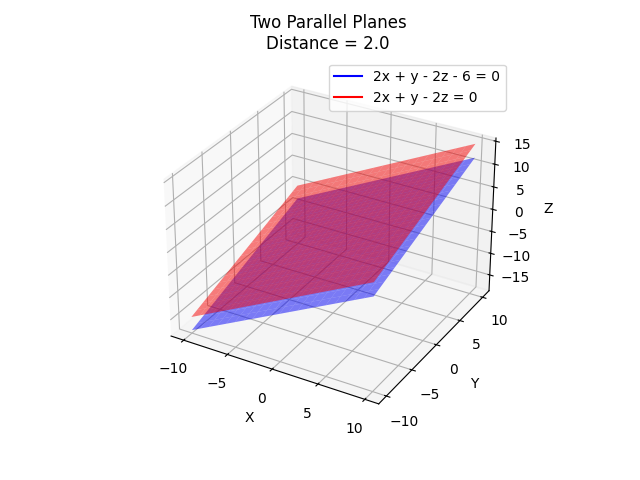
\includegraphics[height=0.5\textheight, keepaspectratio]{figs/Figure_1.png}
    \label{figure_1}
\end{figure}


\end{document}
